\documentclass{standalone}
\usepackage{tikz}
\usetikzlibrary{patterns}
\usetikzlibrary{positioning}
\usetikzlibrary{patterns, positioning}
\usetikzlibrary{shapes.misc}
\usepackage[outline]{contour}
\contourlength{1.5pt} 
\usepackage[sfdefault]{ClearSans}

\begin{document}
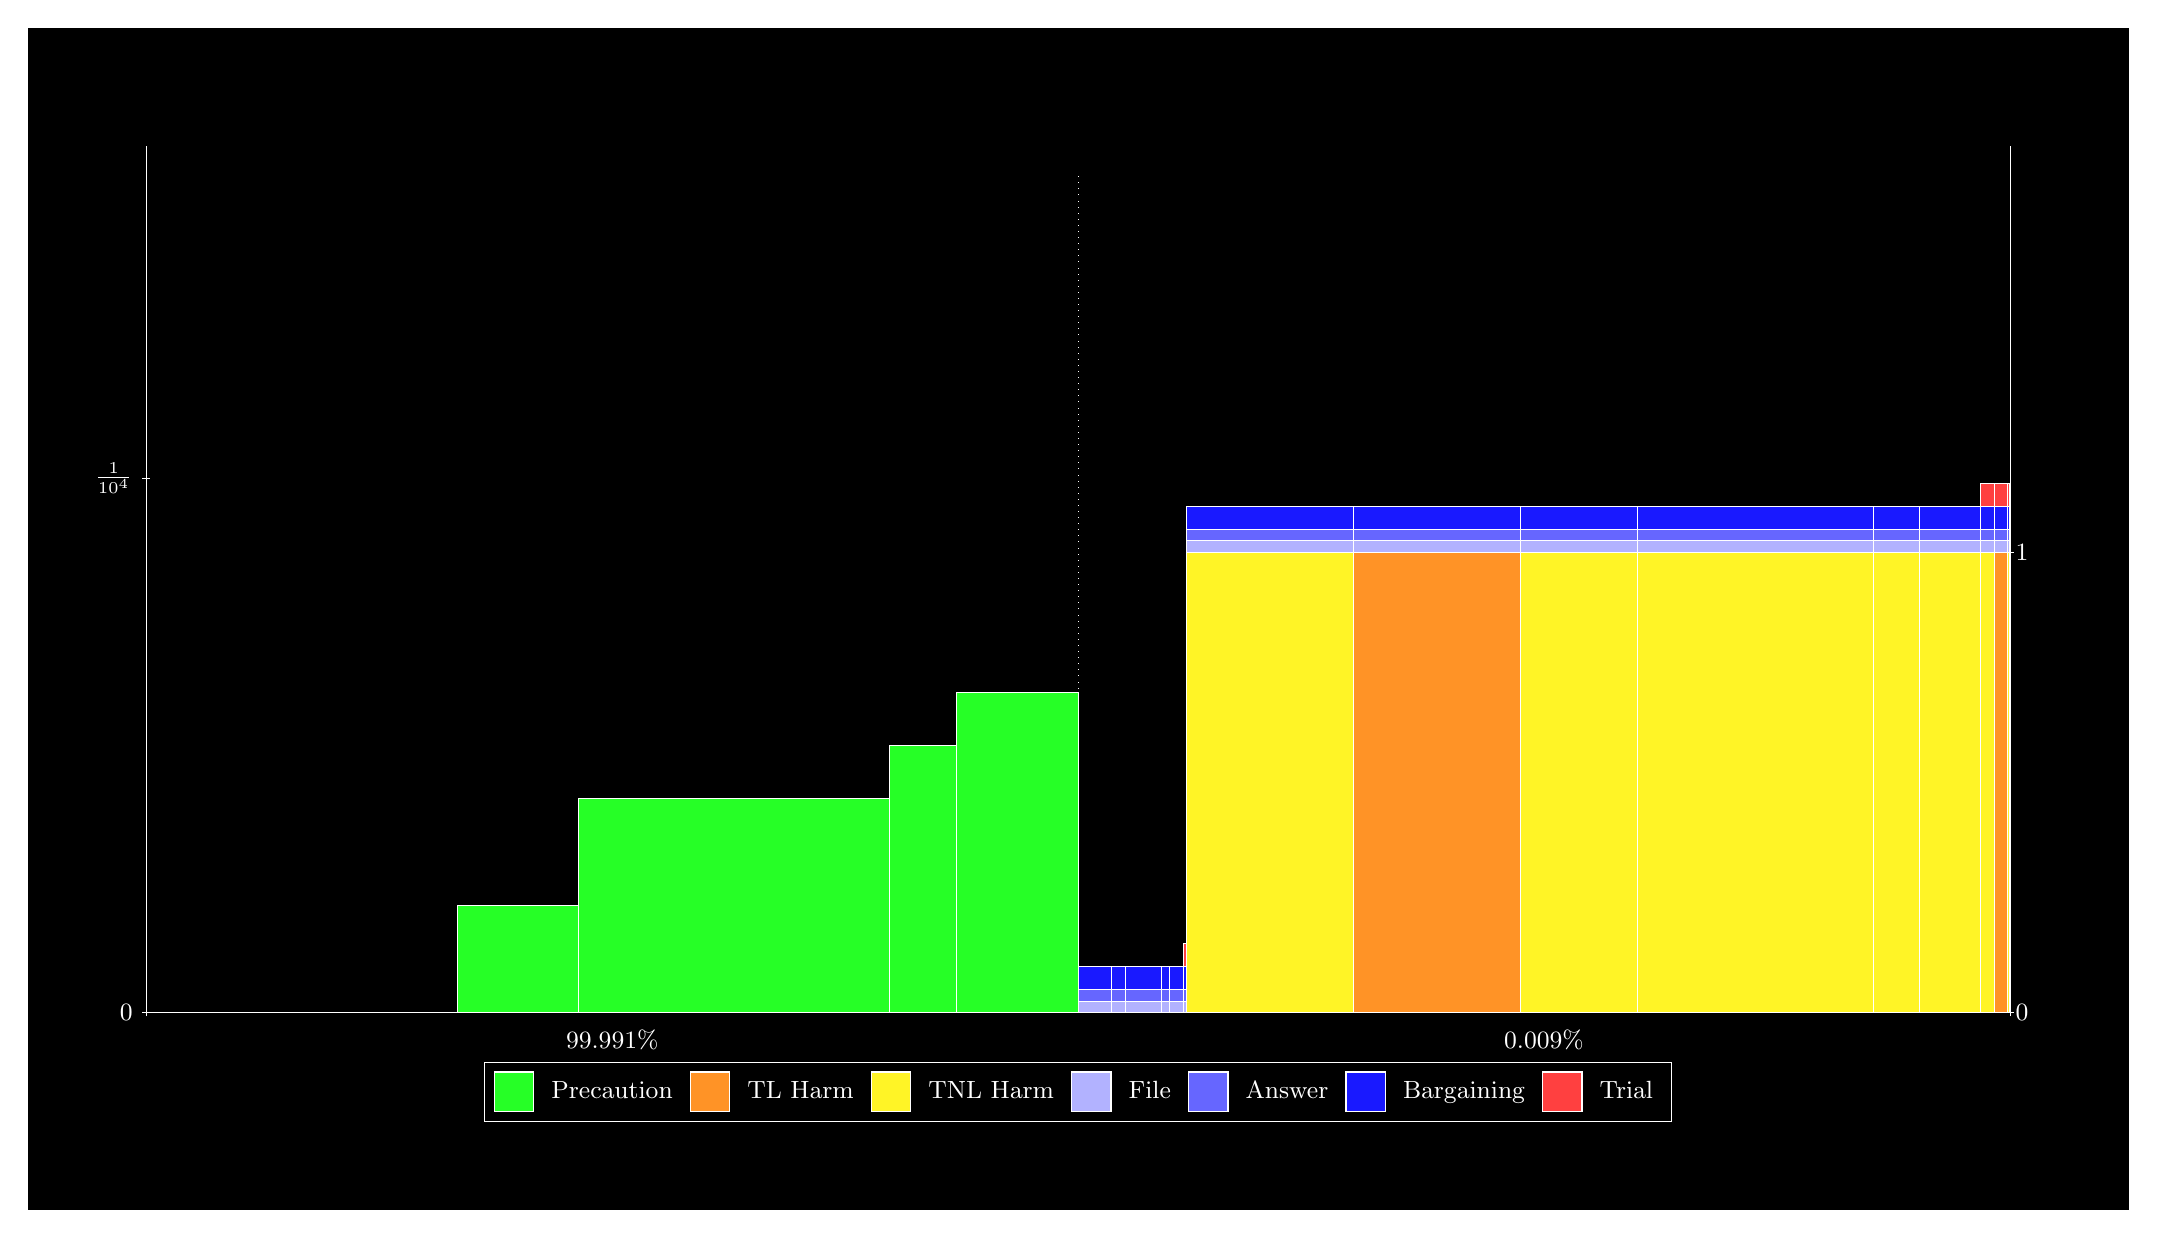
\begin{tikzpicture}
\draw[fill=black] (0,0) rectangle (26.667,15);
\draw[fill=green!85,draw=white,very thin] (5.4443,2.5) rectangle (6.9913,3.8575);
\draw[fill=green!85,draw=white,very thin] (6.9913,2.5) rectangle (10.936,5.2151);
\draw[fill=green!85,draw=white,very thin] (10.936,2.5) rectangle (11.786,5.8939);
\draw[fill=green!85,draw=white,very thin] (11.786,2.5) rectangle (13.333,6.5726);
\draw[fill=blue!30,draw=white,very thin] (13.333,2.5) rectangle (13.758,2.6461);
\draw[fill=blue!60,draw=white,very thin] (13.333,2.6461) rectangle (13.758,2.7923);
\draw[fill=blue!90,draw=white,very thin] (13.333,2.7923) rectangle (13.758,3.0845);
\draw[fill=green!85,draw=white,very thin] (13.758,2.5) rectangle (13.933,2.5001);
\draw[fill=blue!30,draw=white,very thin] (13.758,2.5001) rectangle (13.933,2.6463);
\draw[fill=blue!60,draw=white,very thin] (13.758,2.6463) rectangle (13.933,2.7924);
\draw[fill=blue!90,draw=white,very thin] (13.758,2.7924) rectangle (13.933,3.0847);
\draw[fill=green!85,draw=white,very thin] (13.933,2.5) rectangle (14.391,2.5002);
\draw[fill=blue!30,draw=white,very thin] (13.933,2.5002) rectangle (14.391,2.6464);
\draw[fill=blue!60,draw=white,very thin] (13.933,2.6464) rectangle (14.391,2.7925);
\draw[fill=blue!90,draw=white,very thin] (13.933,2.7925) rectangle (14.391,3.0848);
\draw[fill=green!85,draw=white,very thin] (14.391,2.5) rectangle (14.49,2.5003);
\draw[fill=blue!30,draw=white,very thin] (14.391,2.5003) rectangle (14.49,2.6464);
\draw[fill=blue!60,draw=white,very thin] (14.391,2.6464) rectangle (14.49,2.7926);
\draw[fill=blue!90,draw=white,very thin] (14.391,2.7926) rectangle (14.49,3.0848);
\draw[fill=green!85,draw=white,very thin] (14.49,2.5) rectangle (14.672,2.5004);
\draw[fill=blue!30,draw=white,very thin] (14.49,2.5004) rectangle (14.672,2.6465);
\draw[fill=blue!60,draw=white,very thin] (14.49,2.6465) rectangle (14.672,2.7926);
\draw[fill=blue!90,draw=white,very thin] (14.49,2.7926) rectangle (14.672,3.0849);
\draw[fill=blue!30,draw=white,very thin] (14.672,2.5) rectangle (14.705,2.6461);
\draw[fill=blue!60,draw=white,very thin] (14.672,2.6461) rectangle (14.705,2.7923);
\draw[fill=blue!90,draw=white,very thin] (14.672,2.7923) rectangle (14.705,3.0845);
\draw[fill=red!75,draw=white,very thin] (14.672,3.0845) rectangle (14.705,3.3768);
\draw[fill=yellow!85,draw=white,very thin] (14.705,2.5) rectangle (16.828,8.3455);
\draw[fill=blue!30,draw=white,very thin] (14.705,8.3455) rectangle (16.828,8.4916);
\draw[fill=blue!60,draw=white,very thin] (14.705,8.4916) rectangle (16.828,8.6378);
\draw[fill=blue!90,draw=white,very thin] (14.705,8.6378) rectangle (16.828,8.93);
\draw[fill=orange!85,draw=white,very thin] (16.828,2.5) rectangle (18.95,8.3455);
\draw[fill=blue!30,draw=white,very thin] (16.828,8.3455) rectangle (18.95,8.4916);
\draw[fill=blue!60,draw=white,very thin] (16.828,8.4916) rectangle (18.95,8.6378);
\draw[fill=blue!90,draw=white,very thin] (16.828,8.6378) rectangle (18.95,8.93);
\draw[fill=green!85,draw=white,very thin] (18.95,2.5) rectangle (20.437,2.5001);
\draw[fill=yellow!85,draw=white,very thin] (18.95,2.5001) rectangle (20.437,8.3456);
\draw[fill=blue!30,draw=white,very thin] (18.95,8.3456) rectangle (20.437,8.4917);
\draw[fill=blue!60,draw=white,very thin] (18.95,8.4917) rectangle (20.437,8.6379);
\draw[fill=blue!90,draw=white,very thin] (18.95,8.6379) rectangle (20.437,8.9302);
\draw[fill=green!85,draw=white,very thin] (20.437,2.5) rectangle (20.441,2.5001);
\draw[fill=orange!85,draw=white,very thin] (20.437,2.5001) rectangle (20.441,8.3456);
\draw[fill=blue!30,draw=white,very thin] (20.437,8.3456) rectangle (20.441,8.4917);
\draw[fill=blue!60,draw=white,very thin] (20.437,8.4917) rectangle (20.441,8.6379);
\draw[fill=blue!90,draw=white,very thin] (20.437,8.6379) rectangle (20.441,8.9302);
\draw[fill=green!85,draw=white,very thin] (20.441,2.5) rectangle (23.433,2.5002);
\draw[fill=yellow!85,draw=white,very thin] (20.441,2.5002) rectangle (23.433,8.3457);
\draw[fill=blue!30,draw=white,very thin] (20.441,8.3457) rectangle (23.433,8.4919);
\draw[fill=blue!60,draw=white,very thin] (20.441,8.4919) rectangle (23.433,8.638);
\draw[fill=blue!90,draw=white,very thin] (20.441,8.638) rectangle (23.433,8.9303);
\draw[fill=green!85,draw=white,very thin] (23.433,2.5) rectangle (24.018,2.5003);
\draw[fill=yellow!85,draw=white,very thin] (23.433,2.5003) rectangle (24.018,8.3458);
\draw[fill=blue!30,draw=white,very thin] (23.433,8.3458) rectangle (24.018,8.4919);
\draw[fill=blue!60,draw=white,very thin] (23.433,8.4919) rectangle (24.018,8.6381);
\draw[fill=blue!90,draw=white,very thin] (23.433,8.6381) rectangle (24.018,8.9303);
\draw[fill=green!85,draw=white,very thin] (24.018,2.5) rectangle (24.797,2.5004);
\draw[fill=yellow!85,draw=white,very thin] (24.018,2.5004) rectangle (24.797,8.3458);
\draw[fill=blue!30,draw=white,very thin] (24.018,8.3458) rectangle (24.797,8.492);
\draw[fill=blue!60,draw=white,very thin] (24.018,8.492) rectangle (24.797,8.6381);
\draw[fill=blue!90,draw=white,very thin] (24.018,8.6381) rectangle (24.797,8.9304);
\draw[fill=yellow!85,draw=white,very thin] (24.797,2.5) rectangle (24.965,8.3455);
\draw[fill=blue!30,draw=white,very thin] (24.797,8.3455) rectangle (24.965,8.4916);
\draw[fill=blue!60,draw=white,very thin] (24.797,8.4916) rectangle (24.965,8.6378);
\draw[fill=blue!90,draw=white,very thin] (24.797,8.6378) rectangle (24.965,8.93);
\draw[fill=red!75,draw=white,very thin] (24.797,8.93) rectangle (24.965,9.2223);
\draw[fill=orange!85,draw=white,very thin] (24.965,2.5) rectangle (25.133,8.3455);
\draw[fill=blue!30,draw=white,very thin] (24.965,8.3455) rectangle (25.133,8.4916);
\draw[fill=blue!60,draw=white,very thin] (24.965,8.4916) rectangle (25.133,8.6378);
\draw[fill=blue!90,draw=white,very thin] (24.965,8.6378) rectangle (25.133,8.93);
\draw[fill=red!75,draw=white,very thin] (24.965,8.93) rectangle (25.133,9.2223);
\draw[fill=green!85,draw=white,very thin] (25.133,2.5) rectangle (25.161,2.5001);
\draw[fill=yellow!85,draw=white,very thin] (25.133,2.5001) rectangle (25.161,8.3456);
\draw[fill=blue!30,draw=white,very thin] (25.133,8.3456) rectangle (25.161,8.4917);
\draw[fill=blue!60,draw=white,very thin] (25.133,8.4917) rectangle (25.161,8.6379);
\draw[fill=blue!90,draw=white,very thin] (25.133,8.6379) rectangle (25.161,8.9302);
\draw[fill=red!75,draw=white,very thin] (25.133,8.9302) rectangle (25.161,9.2224);
\draw[fill=green!85,draw=white,very thin] (25.161,2.5) rectangle (25.167,2.5001);
\draw[fill=orange!85,draw=white,very thin] (25.161,2.5001) rectangle (25.167,8.3456);
\draw[fill=blue!30,draw=white,very thin] (25.161,8.3456) rectangle (25.167,8.4917);
\draw[fill=blue!60,draw=white,very thin] (25.161,8.4917) rectangle (25.167,8.6379);
\draw[fill=blue!90,draw=white,very thin] (25.161,8.6379) rectangle (25.167,8.9302);
\draw[fill=red!75,draw=white,very thin] (25.161,8.9302) rectangle (25.167,9.2224);
\draw[white,very thin] (1.5,2.5) -- (1.5,13.5);
\draw[white,very thin] (1.45,2.5) -- (1.55,2.5);
\node[font=\small,text=white, anchor=east] at (1.45, 2.5) {0};
\draw[white,very thin] (1.45,9.2877) -- (1.55,9.2877);
\node[font=\small,text=white, anchor=east] at (1.45, 9.2877) {$\frac{1}{10^{4}}$};

\draw[white,dotted,very thin] (13.333,2.83) -- (13.333,13.17);
\draw[white,very thin] (25.167,2.5) -- (25.167,13.5);
\draw[white,very thin] (25.117,2.5) -- (25.217,2.5);
\node[font=\small,text=white, anchor=west] at (25.117, 2.5) {0};
\draw[white,very thin] (25.117,8.3455) -- (25.217,8.3455);
\node[font=\small,text=white, anchor=west] at (25.117, 8.3455) {1};

\draw[white,very thin] (1.5,2.5) -- (25.167,2.5);
\draw[white,very thin] (1.5,2.45) -- (1.5,2.55);
\node[font=\small,text=white, anchor=north] at (1.5, 2.45) {};
\draw[white,very thin] (25.167,2.45) -- (25.167,2.55);
\node[font=\small,text=white, anchor=north] at (25.167, 2.45) {};

\node[font=\small,text=white,anchor=south] at (7.4167, 1.9) {99.991\%};
\node[font=\small,text=white,anchor=south] at (19.25, 1.9) {0.009\%};
\draw (13.3333,2.5) node (B) {};
\begin{scope}[align=center]
\matrix[scale=0.5,draw=white,below=0.5cm of B,nodes={draw},column sep=0.1cm]{
\node[rectangle,draw,minimum width=0.5cm,minimum height=0.5cm,fill=green!85]{}; & \node[draw=none,font=\small,text=white]{Precaution}; &
\node[rectangle,draw,minimum width=0.5cm,minimum height=0.5cm,fill=orange!85]{}; & \node[draw=none,font=\small,text=white]{TL Harm}; &
\node[rectangle,draw,minimum width=0.5cm,minimum height=0.5cm,fill=yellow!85]{}; & \node[draw=none,font=\small,text=white]{TNL Harm}; &
\node[rectangle,draw,minimum width=0.5cm,minimum height=0.5cm,fill=blue!30]{}; & \node[draw=none,font=\small,text=white]{File}; &
\node[rectangle,draw,minimum width=0.5cm,minimum height=0.5cm,fill=blue!60]{}; & \node[draw=none,font=\small,text=white]{Answer}; &
\node[rectangle,draw,minimum width=0.5cm,minimum height=0.5cm,fill=blue!90]{}; & \node[draw=none,font=\small,text=white]{Bargaining}; &
\node[rectangle,draw,minimum width=0.5cm,minimum height=0.5cm,fill=red!75]{}; & \node[draw=none,font=\small,text=white]{Trial}; \\\\
};\end{scope}

\end{tikzpicture}
\end{document}